\newpage
\section{Sistema Pipeline}
Una architettura pipeline è una tipologia di soluzione che viene implementata internamente nei processori per permettere l'esecuzione parallela di più istruzioni.
Per comprendere meglio cosa si intende per esecuzione parallela di più istruzioni, andiamo a considerare la strutturazione interna del flusso di esecuzione di una normale istruzione. L'esecuzione si divide nelle seguenti fasi (visualizzabili anche alla figura [\ref{img:pipe}]):
\begin{itemize}
    \item \textbf{Istruction Fetch (IF)}: Ovvero il prelievo dell'istruzione dalla memoria;
    \item \textbf{Decode (DEC)}: Decodifica ed interpretazione dell'istruzione;
    \item \textbf{Execute (EX)}: Esecuzione effettiva dell'istruzione;
    \item \textbf{Memory write (MW)}: Effettuo il prelievo dei dati all'interno della memoria;
    \item \textbf{Register write (RW)}: Inserisco i dati che mi interessano dai registri, in memoria. 
\end{itemize}

\begin{figure}
    \centering
    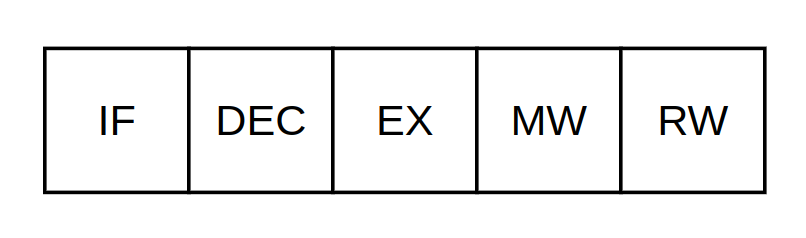
\includegraphics[width=.5\textwidth]{img/Pipeline.png}
    \caption{Architettura classica pipeline (ordine di esecuzione fasi)}\label{img:pipe}
\end{figure}

Definito il flusso di esecuzione di un' istruzione, l'architettura pipeline cerca di eseguire le fasi di un' istruzione in maniera del tutto separata, in modo da poter eseguire più fasi di istruzioni differenti, aumentando il throughput di 5 volte rispetto alla classica architettura sequenziale di Von Neumann. Per capire meglio questo concetto facciamo un esempio:
Devo eseguire un programma che ha 5 istruzioni, allora parto con l'esecuzione della prima fase, che preleverà l'istruzione i1, una volta prelevata, l'istruzione i1 passa alla fase di decode, mente, allo stesso istante, viene caricata l'istruzione i2 (quindi viene effettuata la Istruction Fetch dell'istruzione successiva mentre viene decodificata la precedente). Se eseguiamo tale procedura per tutte le fasi noteremo che ad ogni impulso di clock (a regime), il processore darà un risultato, quindi non ci sarà bisogno di eseguire tutte le istruzioni una per volta, poichè la suddivisione delle fasi ne permette un' esecuzione "parallela" (o meglio dire pipeline).

Per fare in modo di isolare l'esecuzione delle varie fasi, tra i vari blocchetti saranno presenti dei registri, che permettono di conservare lo stato su cui una determinata fase sta lavorando (come le architetture pipeline in elettronica [\ref{img:pipe-reg}]). 

\begin{figure}[!ht]
    \centering
    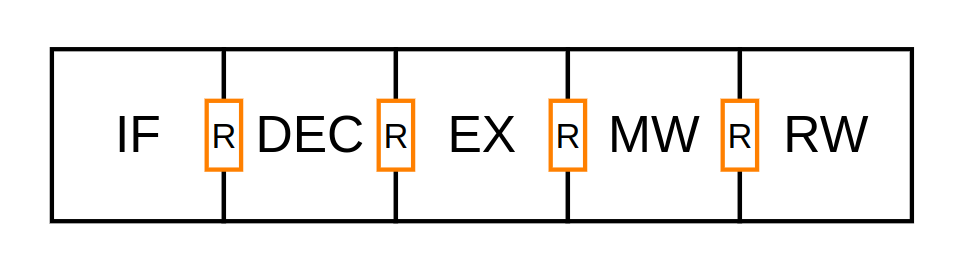
\includegraphics[width=.5\textwidth]{img/Pipe-reg.png}
    \caption{Architettura classica pipeline con registri}\label{img:pipe-reg}
\end{figure}

Esistono tuttavia dei limiti dell'architettura pipeline la cui risoluzione verrà discussa (almeno per quelli che ci riguardano) nei prossimi paragrafi:

\begin{itemize}
    \item \textbf{Vincolo di tempo}: Le fasi presentate operano in pipe, quindi funzionano bene se tutte le unità funzionali impiegano un tempo più o meno costante. Se così non fosse, l'intero processore sarà rallentato dall'unità funzionale più lenta. La condizione di tempo di risposta costante è garantita solo se le istruzioni sono particolarmente semplici (condizione tipica dei sistemi RISC);
    \item \textbf{Vincolo tecnologico}: Tutte le unità funzionali sono pilotate contemporaneamente dallo stesso clock. Il problema tecnologico è che il clock può essere schematizzato elettronicamente come un circuito induttivo/capacitivo, e di conseguenza le ultime unità a percepire il segnale di clock, se la frequenza del treno di impulsi è troppo elevata, troppo \textit{filtrato} (a causa del filtro capacitivo) o troppo rumoroso (a causa dell'effetto induttivo). Questo fenomeno prende il nome di Skew del segnale di clock, e dunque è opportuno adottare delle misure di ridondanza e controllo correttezza a monte di ogni collegamento unità funzionale-clock;
    \item \textbf{Problema delle istruzioni di salto}: Quando si incontra un'istruzione di salto, bisogna eseguirla completamente (fine fase EX), prima di sapere se il salto deve essere effettuato o meno e prima di conoscere l'indirizzo della prossima istruzione da prelevare. La filosofia generale è quella di non fermare la pipe, e quindi continuare a caricare istruzioni in modo sequenziale, e all'occorrenza eliminarle dalla pipe (\textit{branch penalty}) (\ref{par:MIPS_gestione_salti});
    \item \textbf{Problema del conflitto sui dati}: Spesso accade che due istruzioni consecutive cercano di leggere e scrivere contemporaneamente lo stesso registro e ciò potrebbe causare gravi errori. Nei processori CISC i conflitti sui dati sono più probabili, siccome quest’ultimi tendono a garantire tutti i modi di indirizzamento per tutte le istruzioni. Il conflitto sui dati è confinato alle ultime tre fasi: EX, MEM e WB;
    \item \textbf{Problema della gestione delle interruzioni}: In un sistema pipeline è più complesso gesite sia le interruzioni esterne che garantire il corretto ordine di esecuzione delle interruzioni interne;
    \item \textbf{Problema dei conflitti per l'accesso in memoria}: Più fasi possono tentare di accedere contemporaneamente alla memoria, per eseguire operazioni di lettura delle istruzioni o scrittura sui dati. 
\end{itemize}

Un'architettura di questo tipo, però, richiede una serie di ipotesi, ovvero:
\begin{itemize}
    \item Divisione di memoria dati e memoria istruzioni (altrimenti dovrei gestire anche dei conflitti tra l'istruction fetch e la register/memory write);
    \item Le memorie devono garantire degli accessi molto veloci: ad ogni colpo di clock vengono effettuate 5 fasi e potenzialmente scritto un risultato.
    \item Le operazioni artimetico-logiche devono essere effettuate prevalentemente tra i registri interni del processore, condizione che caratterizza fortemente i processori RISC;
    \item Le istruzioni devono avere tutte lunghezza fissa;
\end{itemize}

Guardando le ipotesi possiamo capire che alcune tipologie di operazioni, che solitamente effettuevamo sul processore motorola, ora dovranno essere scompattate in varie operazioni. Un esempio classico è il comando \lstinline|ADD VAR,D1|, che utilizzava l'indirizzamento diretto per il prelievo dell'operando dalla memoria. In questo caso, però, l'indirizzamento diretto non è possibile, poichè si andrebbe ad invalidare un'ipotesi, ovvero, la lunghezza fissa dell'istruzione (che dovrebbe poi contenere l'indirizzo di memoria). Pertanto non sono previsti tutti i modi di indirizzamento.

Per comprendere meglio la problematica, consideriamo di avere un prelievo dalla memoria con un'architettura a 16-bit, ma con il memory address ed il memory buffer a 32-bit. Pertanto il seguente comando non sarebbe possibile: \lstinline|MOVE VAR,D0|; poichè richiederebbe il prelievo dell'indirizzo di memoria da 32-bit dalla memoria, ma per effettuare tale operazione, avendo solo 16 bit, avrei bisogno di due istruzioni che caricano, una i primi 16-bit e l'altra i restanti 16. Tale suddivisione, però non viene fatta dal programmatore, ma dal compilatore. Ci sono varie istruzioni che sono come la MOVE, tali istruzioni sono dette pseudo-istruzioni, poichè il compilatore andrà a suddividerle in più operazioni differenti al fine di raggiungere il risultato desiderato.

Questa cosa ci permette di capire, a questo punto, la suddivisione tra architettura di tipo CISC e architetture di tipo RISC. Le architetture di tipo CISC permettono l'esecuzione di istruzioni che sono più articolate, ma a costo di una complessità architetturale maggiore, mentre nelle architetture RISC, data la semplicità dell'architettura, le tipologie di operazioni che si possono effettuare sono ridotte ma più veloci.

\subsection{Modelli di sistemi pipeline}
Il sistema pipeline, dato il suo sistema di funzionamento, può introdurre varie tipologie di problematiche. Negli anni si sono sviluppate varie tipologie di soluzioni differenti.
Le principali architetture con cui si va a contatto al giorno d'oggi sono:
\begin{itemize}
    \item \textbf{MIPS}: Tipologia di ISA sviluppata da Patterson che poi ha venduto, per cui ora la sua implemetazione è proprietaria;
    \item \textbf{RISC-V}: Tipologia di ISA molto simile al MIPS, ma open-source;
    \item \textbf{ARM}: Tipologia di ISA proprietaria, utilizzatissima in svariati amiti (particolarmente in quello industriale), la cui implementazione è proprietaria;
\end{itemize}

Nel caso particolare di questo corso, andremo a vedere il funzionamento del RISC-V facendo riferimento sempre al MIPS, per cui saranno queste le due tipologie di architetture che si andranno ad approfondire.

Le principali problematiche che bisogna affrontare all'interno di un architettura pipeline sono le seguenti:
\begin{itemize}
    \item \textbf{Interruzioni}: Quando bisogna gestire un' interruzione la gestione dell'architettura pipe si complica, poichè bisogna capire chi ha interrotto e bisogna salvare lo stato di tutte le istruzioni che stanno eseguendo, che risulta una cosa molto onerosa e complicata;
    \item \textbf{Concorrenza sui registi}: Se due istruzioni, devono utilizzare un'informazione presente nello stesso registro ad esempio: R1 = R2+R3; R0=R1+R4;  Notiamo che per eseguire la seconda istruzione vi è bisogno del completamento della prima, ma il risultato effettivo viene scritto solo alla fine del ciclo, per cui si potrebbe incorrere in vari errori;
    \item \textbf{Salti}: Quando devo effettuare un salto, se considero il caso condizionato, non so a quale ramo andrò a saltare, è quindi più complicato capire quale sarà l'istruzione successiva da eseguire;
    \item \textbf{Gestione delle pipe multiple}: ho molteplici pipe di esecuzione, che quindi richiede una loro gestione per prevenire eventuali conflitti;
\end{itemize}

Una delle problematiche che maggiormente incide è quella riguardante il salto, poichè, dato che non conosco quale sia l'istruzione successiva, vado a bloccare la pipe appena noto che ho un'istruzione di salto, ed appena è verificata la condizione, vado a prelevare tale istruzione dalla memoria. Però questa soluzione risulta molto inefficiente, poichè introduce dei periodi in cui la pipe rimane in stallo. Difatti, una soluzione che è stata trovata è quella della branch prediction, per cui vado a processare le istruzioni successive, cercando di prevedere quale sarà il branch da eseguire, solo nel caso in cui mi accorgo che sto sbagliando vado ad effettuare il blocco della pipe, altrimenti continuo con la normale esecuzione del programma.

\subsection{Architettura del MIPS}
Il MIPS (Microprocessor without Interlocked Pipelined Stages) è una tipologia di architettura Pipelined di tipo RISC.
Nel precedente capitolo abbiamo visto le fasi di esecuzione di un'architettura pipelined generale [\ref{img:pipe}], però, nel caso del MIPS, tali fasi variano leggermente. Difatti il MIPS è caratterizzato dalle seguenti fasi:
\begin{itemize}
    \item \textbf{Istruction Fetch}: Prelievo dell'istruzione dalla memoria e incremento del program counter;
    \item \textbf{Decode}: Si vanno a prelevare gli operandi dal \textit{register file} e si preparano i segnali di controllo per la fase di esecuzione. Il register file è una componente fondamentale all'interno di un processore. Si tratta di un insieme organizzato di registri che servono per archiviare temporaneamente dati e istruzioni durante l'esecuzione dei programmi. Supporta operazioni di lettura e scrittura simultanee, infatti il processore può leggere/scrivere da/verso più registri nello stesso ciclo di clock;
    \item \textbf{Execute}: Esecuzione delle operazioni logico-aritmetiche pilotate dai segnali della fase di decode precedente;
    \item \textbf{Memory}: Vado a leggere o scrivere qualcosa dalla memoria e gestione dei salti;
    \item \textbf{Write Back}: Accesso in scrittura al register file per scrivere i risultati ottenuti;
\end{itemize}

\begin{figure}[!ht]
    \centering
    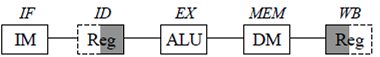
\includegraphics[width=0.25\textwidth]{img/MIPS_clock_split.png}
    \caption{Divisone temporale impulso di clock}
    \label{img:MIPS_divisione_clock}
\end{figure}

Come per tutte le architettura pipelined, anche il MIPS richiede che tra le varie fasi vi siano dei registri che conservino lo stato dell'operazione.
Il MIPS, pertanto, presenta vari casi di conflitto che richiedono delle ipotesi sul sistema stesso. Tali ipotesi sono:

\begin{itemize}
    \item \textbf{Velocità della memoria}: La memoria che sarà utilizzata dal MIPS sarà acceduta molto frequentemente (precisamente 5 volte in più rispetto al caso senza pipe);
    \item \textbf{Concorrenze sulla memoria}: Presenza di due memorie, una per le istruzioni ed una per i dati. Tali memorie vengono previste per evitare la concorrenza tra la fase di fetch (prelievo dell'istruzione dalla memoria) e la fase di MEM (lettura o scrittura dalla memoria);
    \item \textbf{Concorrenza sui registri}: Potenzialmente sul register file possono verificarsi dei conflitti, in particolare quando contemporaneamente un'istruzione vi accede in lettura e una in scrittura. Per risolvere il conflitto, le operazioni di lettura e scrittura vengono effettuate in due intervalli separati dello stesso ciclo di clock, e in particolare la fase di decode (lettura) opera nella seconda parte del ciclo di clock, mentre la fase di write back (scrittura) opera nella prima parte, come riportato in figura \ref{img:MIPS_divisione_clock};
\end{itemize}

\begin{figure}[!ht]
    \centering
    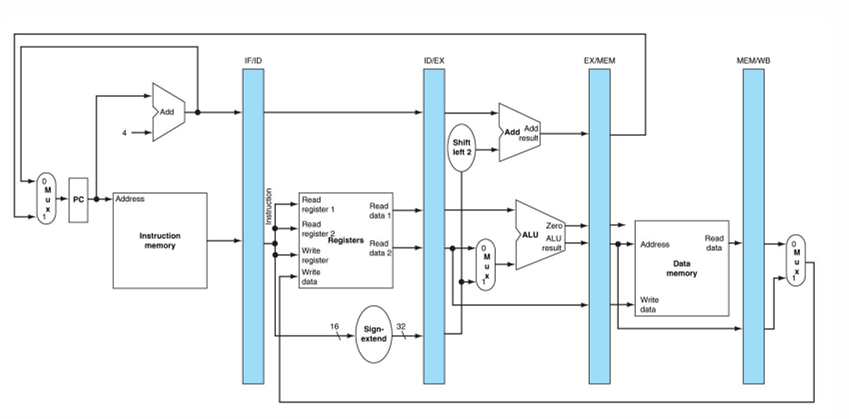
\includegraphics[width=0.75\textwidth]{img/MIPS_architettura_pipeline.png}
    \caption{Architettura della pipeline MIPS}
    \label{img:MIPS_architettura_pipeline}
\end{figure}

\subsubsection{Fase di Fetch}
La fase di fetch è caratterizzata da 2 principali operazioni, la fase di prelievo dell'indirizzo e la fase di incremento del program counter. 
L'istruzione viene letta dalla Instruction memory, indirizzata al PC e posta nel registro di comunicazione tra fase IF e fase ID. Dopodichè, il PC viene incrementato e copiato nel registro di comunicazione, perchè potrebbe, nel caso di istruzioni di salto, servire a fasi successive.
Pertanto la sua parte architetturale è formata dalle componenti:
\begin{itemize}
    \item \textbf{ADD}: Al fine di favorire l'indipendenza dell'incremento del PC (operazione che avviene con la massima frequenza), l'operazione viene effettuata da un circuito dedicato, in modo da calcolare il prossimo indirizzo del PC senza interferire con altre operazioni dell'ALU principale, in modo da prevenire conflitti sulla pipe;
    \item \textbf{MUX}: Seleziona se considerare l'indirizzo di memoria successivo del program counter o un registro di memoria dettato dalla fase di MEM (caso di istruzioni di salto);
    \item \textbf{PC}: Registro program counter;
    \item \textbf{Istruction Memory}: Prelievo dell'istruzione da eseguire dalla memoria;
\end{itemize}

\subsection{Fase di Decode}
Nella fase di Decode, il MIPS, va a decodificare ed interpretare il comando. In particolare, vengono letti gli eventuali registri sorgente (nel caso di indirizzamento Register o Immediato) dal register file e memorizzati nel registro di comunicazione ID/EX. Nel caso di istruzioni con indirizzamento Immediato, i 16 bit del valore vengono convertiti in un valore a 32 bit estendendo il segno, e il valore così esteso viene inserito nel registro di comunicazione. Inoltre, il valore del PC precedentemente passato dalla fase di IF, viene propagato insieme alle altre informazioni al registro di comunicazione successivo. Osserviamo che il numero di registro destinazione in cui memorizzare un dato nella fase WB deve essere propagato lungo tutta la pipeline.
Le parti che compongono l'architettura della fase di decode dunque sono:
\begin{itemize}
    \item \textbf{Registers}: Registri interni del processore che possono essere pilotati sia in lettura che in scrittura tramite dei segnali esterni (contenuti nella sotto-architettura);
    \item \textbf{Sign-extend}: Blocco di estensione con segno dei possibili valori immediati contenuti nell'istruzione;
\end{itemize}

Il blocco estensione del segno è fondamentale perchè l'architettura MIPS utilizza istruzioni di lunghezza fissa di 32 bit per semplificare il design del processore e migliorare la velocità di decodifica, e dunque la codifica dei valori acceduti con indirizzamento immediato è fissata a 16 bit. L'estensione a 32 bit è necessaria perchè garantisce che il valore immediato possa essere direttamente utilizzato per le operazioni aritmetiche o logiche con i registri (che sono anch'essi a 32 bit).

\subsection{Fase di Execute}
Nella fase Execute viene eseguita effettivamente l'istruzione. In particolare, vengono prelevati i dati e i bit di controllo dal registro ID/EX e vengono effettuate le oeprazioni logico-aritmetiche dalla ALU, e i risultati vengono memorizzati nel registro di comunicazione EX/MEM. In caso di istruzioni di salto, viene presa la decisione di saltare o meno, e viene calcolato il nuovo valore di PC, che viene inserito nel registro di comunicazione EX/MEM. In caso di istruzioni load/store, viene calcolato l'indirizzo dell'operando in memoria e posto in EX/MEM. 
La parte architetturale è composta da vari componenti interessanti.
\begin{itemize}
    \item \textbf{Add}: Strumento che viene utilizzato per calcolare un eventuale offset rispetto ad un valore, e viene utilizzato per calcolare il nuovo valore del PC in caso di salti condizionati o incondizionati;
    \item \textbf{Shift left 2}: Moltiplica per 4 il valore per cui voglio saltare (in modo da saltare a 4 indirizzi più avanti);
    \item \textbf{ALU}: Strumento di calcolo aritmetico-logico;
    \item \textbf{Multiplexer}: Seleziona o il dato immediato o un secondo dato proveniente da un registro, proveniente dalla fase precedente;
\end{itemize}

\subsection{Fase di Mem}
Nella fase di memorizzazione avviene l'accesso alla memoria dati, secondo l'indirizzo comunicato dalla fase precedente nel registro EX/MEM. In caso di istruzione di LOAD, il dato viene letto e propagato nel registro MEM/WB. 
La sua architettura è composta principalmente dal singolo elemento di accesso alla memoria dati.

\subsection{Fase di Write Back}
In tale fase vado a verificare cosa bisogna scrivere all'interno dei registri interni. Il componente che meglio indica il suo funzionamento è il multiplexer finale che serve per specificare se il dato da caricare all'interno dei registri sia il risultato dell'ALU o qualche valore proveniente dalla memoria dati. 

\subsection{Registri Intermedi}
I registri che sono posti tra una fase e l'altra della pipeline sono molto più complessi di quel che si crede. Essi non contengono solo dati informativi (operandi e risultati), ma contengono anche: traccia dell'operazione da effetture, destinazione del risultato ecc. 
L'architettura e le componenti di cui si è parlato sopra, quindi, sono solo una parte di quello che è effettivamente stato realizzato sull'hardware del dispositivo.
La schematizzazione che abbiamo fatto ci permette di capire bene il funzionamento di un sistema pipeline senza entrare troppo nei dettagli della sua implementazione hardware.

\subsection{Gestione dei Salti} \label{par:MIPS_gestione_salti}
L'architettura pipeline ha una criticità di cui abbiamo già attentamente discusso in precedenza, i salti. 
Quando sopraggiunge un istruzione di salto, riusciamo a captare che è così solo nella fase di esecuzione dell'istruzione, mentre la pipe ha continuato a caricare le istruzioni in modo sequenziale, che si troveranno rispettivamente nella fase di IF e ID e non avranno quindi ancora modificato lo stato del processore e della memoria. Nel caso in cui il salto non deve essere eseguito, allora la pipe continuerà a funzionare normalmente, mentre se il salto deve essere eseguito, le istruzioni caricate dovranno essere eliminate dalla pipe (\textit{pipe flush}) e dovrà essere caricata l'istruzione a cui punta il salto e le successive. Il ritardo che segue quest'ultimo caso è detto \textit{branch penalty}. L'obiettivo è quello di confinare la gestione dei salti nelle fasi IF e ID, perchè in quelle fasi le istruzioni non hanno ancora modificato lo stato del processore e della memoria, e quindi la rete di controllo hardware deve riguardare solo queste due fasi.
In generale, il problema è risolvibile fondamentalmente mediante due approcci: l'approccio conservativo e l'approccio ottimistico (\textit{branch prediction}).
Nel caso dell'approccio conservativo, quando il processore interpreta durante la fase ID un'istruzione come istruzione di salto, ferma la pipe e disabilita la propagazione dell'istruzione che si trova erroneamente nella fase IF, determina l'istruzione a cui saltare in fase EX e la preleva. Si torna insomma al modello sequenziale di Von Neumann. Il conto è salato se consideriamo che le istruzioni di salto costituiscono il 25\% di un programma, e infatti ne consegue un notevole spreco delle risorse di parallelismo fornite dalla pipe. Questo approccio è \textit{leggermente} migliorabile attraverso l'hardware, anticipando la decisione inerente al salto alla fase di ID, in base alla condizione di salto. Ad esempio l'istruzione \lstinline|JNZ <LABEL>| controlla se il flag Z del SR è alto, e in tal caso non occorre saltare e quindi l'istruzione che si è prelevata nel frattempo è giusta. Molti ritardi possono essere  evitati dal programmatore o dal compilatore: il programmatore può contribuire al buon funzionamento del sistema, scrivendo le istruzioni in un ordine tale da minimizzare le probabilità di stallo della pipe. Nel caso di un costrutto if-then-else, ad esempio, conviene inserire nel ramo then l'alternativa più probabile. Il compilatore, da parte sua, può operare vari accorgimenti; ad esempio, siccome un ciclo for è sempre tradotto in un if-then-else, esso deve inserire l'alternativa più probabile nel ramo then.
In fase di compilazione è possibile evitare l'approccio conservativo. Se immediatamente prima del salto c'è un'istruzione con operandi da cui non dipende l'esito della scelta di saltare o meno, è possibile in fase di compilazione inserire l'istruzione indipendente dopo il branch, in modo da sfruttare lo slot di tempo in cui l'istruzione viene caricata ed entra nella pipe, e quindi non c'è bisogno di pipe flush. Qualora non sia possibile invertire una istruzione if con quella che la precede, il compilatore potrebbe decidere di mettere subito dopo la if una \textbf{nop}, istruzione che non ha alcun effetto e quindi non è mai errato inserirla nella pipe. In questo modo si può operare senza considerare alcun tipo di approccio. Possiamo aggiungere che se stiamo considerando un'istruzione di salto in un processore CISC con una condizione di salto elaborata, allora il numero di nop che bisogna inserire a seguito dell'istruzione di salto risulta essere superiore a 1, in quanto ricordiamo che la pipe per i CISC è più lunga e la valutazione della condizione coinvolge più fasi oltre le prime due, di caricamento e decodifica.
Una soluzione meno conservativa a quella appena presentata è di utilizzare la \textbf{branch-prediction} (approccio ottimistico).

% Per Agostino: Ho cambiato interamente questa sezione in accordo agli appunti di de Benedictis, molto più sensati e chiari di quanto farfugliato a lezione.


% e quindi, se dovessimo aggiustare il PC seguendo tutta la pipe, dovremmo aspettare la fase di write back. L'obiettivo è quello di confinare la gestione dei salti nelle fasi IF e ID, perchè in quelle fasi le istruzioni non hanno ancora modificato lo stato del processore e della memoria, e quindi la rete di controllo hardware deve riguardare solo queste due fasi. Per evitare tale situazione di inefficienza, andiamo a retroazionare la fase di esecuzione con la fase di Istruction Fetch. Tale retroazione permette di capire quando e dove poi si andrà a saltare. Ciò però deve prevedere il sacrificio o l'introduzione di un istruzione "vittima", tale istruzione sarà eseguita indipendentemente a dove si andrà a saltare. Tale istruzione è la no-operation (NOP), che viene inserita subito dopo la JMP per evitare la perdita di eventuali istruzioni utili.
% Tale soluzione è molto buona quando lavoro con il MIPS, poichè questo è caratterizzato dalla sua particolare pipe molto corta (e quindi molto RISC), ma nei processori più moderni, posso avere delle pipe molto più profonde ed articolate. 

\subsubsection{Branch prediction}
La branch prediction è una tecnica che cerca di prevedere a quale ramo un istruzione di salto condizionato possa saltare. Tale tecnica valuta le prestazioni in base a quanto si possa "perdere" in termini di efficienza (ricaricare il branch corretto rispetto a quello predetto).
Per capire bene questa cosa andiamo a considerare il seguente pseudocodice:
\begin{lstlisting}[language=C]
for (int i = 0; i < N; i++){
    for (int j = 0; j < N; j++){
        operazioni
    }
}
\end{lstlisting}

Tali for prevedono un controllo iniziale sulla variabile. Vedendo come sono strutturati tale controllo prevede l'esecuzione del ramo else una sola volta (guardando il for interno) ogni N passi.
I modi pre prevedere il branch possono essere vari, e possono essere descritti mediante degli appositi automi a stati finiti. Un primo approccio molto basilare è quello di andare a cambiare il branch da caricare successivamente ad ogni errore di decisione e quindi eseguire le operazioni descritte dall'automa [\ref{img:automa-semplice}].

\begin{figure}[!ht]
    \centering
    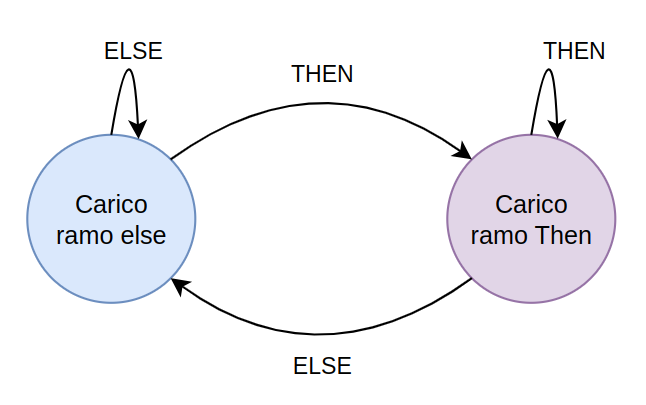
\includegraphics[width=.5\textwidth]{img/automa-semplice.png}
    \caption{Automa della branch prediction base}\label{img:automa-semplice}
\end{figure}

Tale soluzione, però, guardando al nostro caso, non è proprio ottimale, poichè per quel singolo fail che avviene ad ogni N interazioni dovrò assorbirmi 2 fault. Per evitare tale condizione, e quindi rendere la persistenza più forte, vado a costruire un automa a 4 stati che mi permette di rendere la condizione di "cambio del branch" più solida, poichè solo in caso di due fault successivi (fault = errore nel riconoscere il branch giusto), allora cambio il mio branch effettivo. L'automa che meglio spiega tale principio è quello visualizzabille all'immagine [\ref{img:automa-complesso}]

\begin{figure}[!ht]
    \centering
    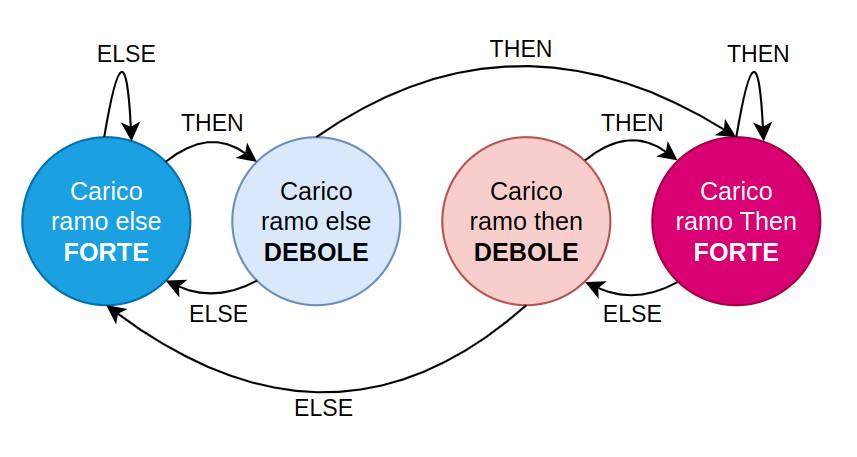
\includegraphics[width=.5\textwidth]{img/automa-complesso.png}
    \caption{Automa della branch prediction avanzato}\label{img:automa-complesso}
\end{figure}

Per implementare la predizione a livello hardware, il processore utilizza una \textbf{tabella di predizione} dei salti. Una possibile struttura è la seguente.
\begin{itemize}
    \item Indirizzo dell'istruzione di salto.
    \item Indirizzo di destinazione (dove saltare).
    \item 2 Bit per codificare lo stato dell'automa.
\end{itemize}

La tabella viene aggiornata in parallelo durante la fase di Execute (EX), ovvero nel momento in cui il processore verifica se la predizione è corretta. Se c'è stato un errore, si aggiorna lo stato dell'automa (e la corrispondente voce nella tabella). Tale struttura è memorizzata in un apposita area di memoria, detta \textbf{Branch History Table} (BHT).
\\
\\
Cerchiamo di capire come sia possibile realizzare una memoria dalle caratteristiche descritte in precedenza. Osserviamo innanzitutto che un tale funzionamento non può essere ottenuto da un classico schema di MUX e DEMUX, in quanto l'ingresso della memoria sarà una chiave (indirizzo 100) e l'uscita sarà un valore (indirizzo 104 o 104). Per cui, la memoria si compone di una serie di chiavi, a ognuna delle quali viene associata un'informazione. \MakeUppercase{è} inoltre presente un comparatore legato a ciascuna chiave, che restituisce un valore alto se questa coincide con il valore della chiave fornito in ingresso. Tutte le informazioni memorizzate sono collegate a un MUX, che viene pilotato dalle uscite dei comparatori. Una tale tipologia di memoria è detta \textbf{associativa} [\ref{fig:mem_associativa}], e differisce dalle classiche memorie indirizzabili quali, RAM o hard disk.
\begin{figure}[!h]
    \centering
    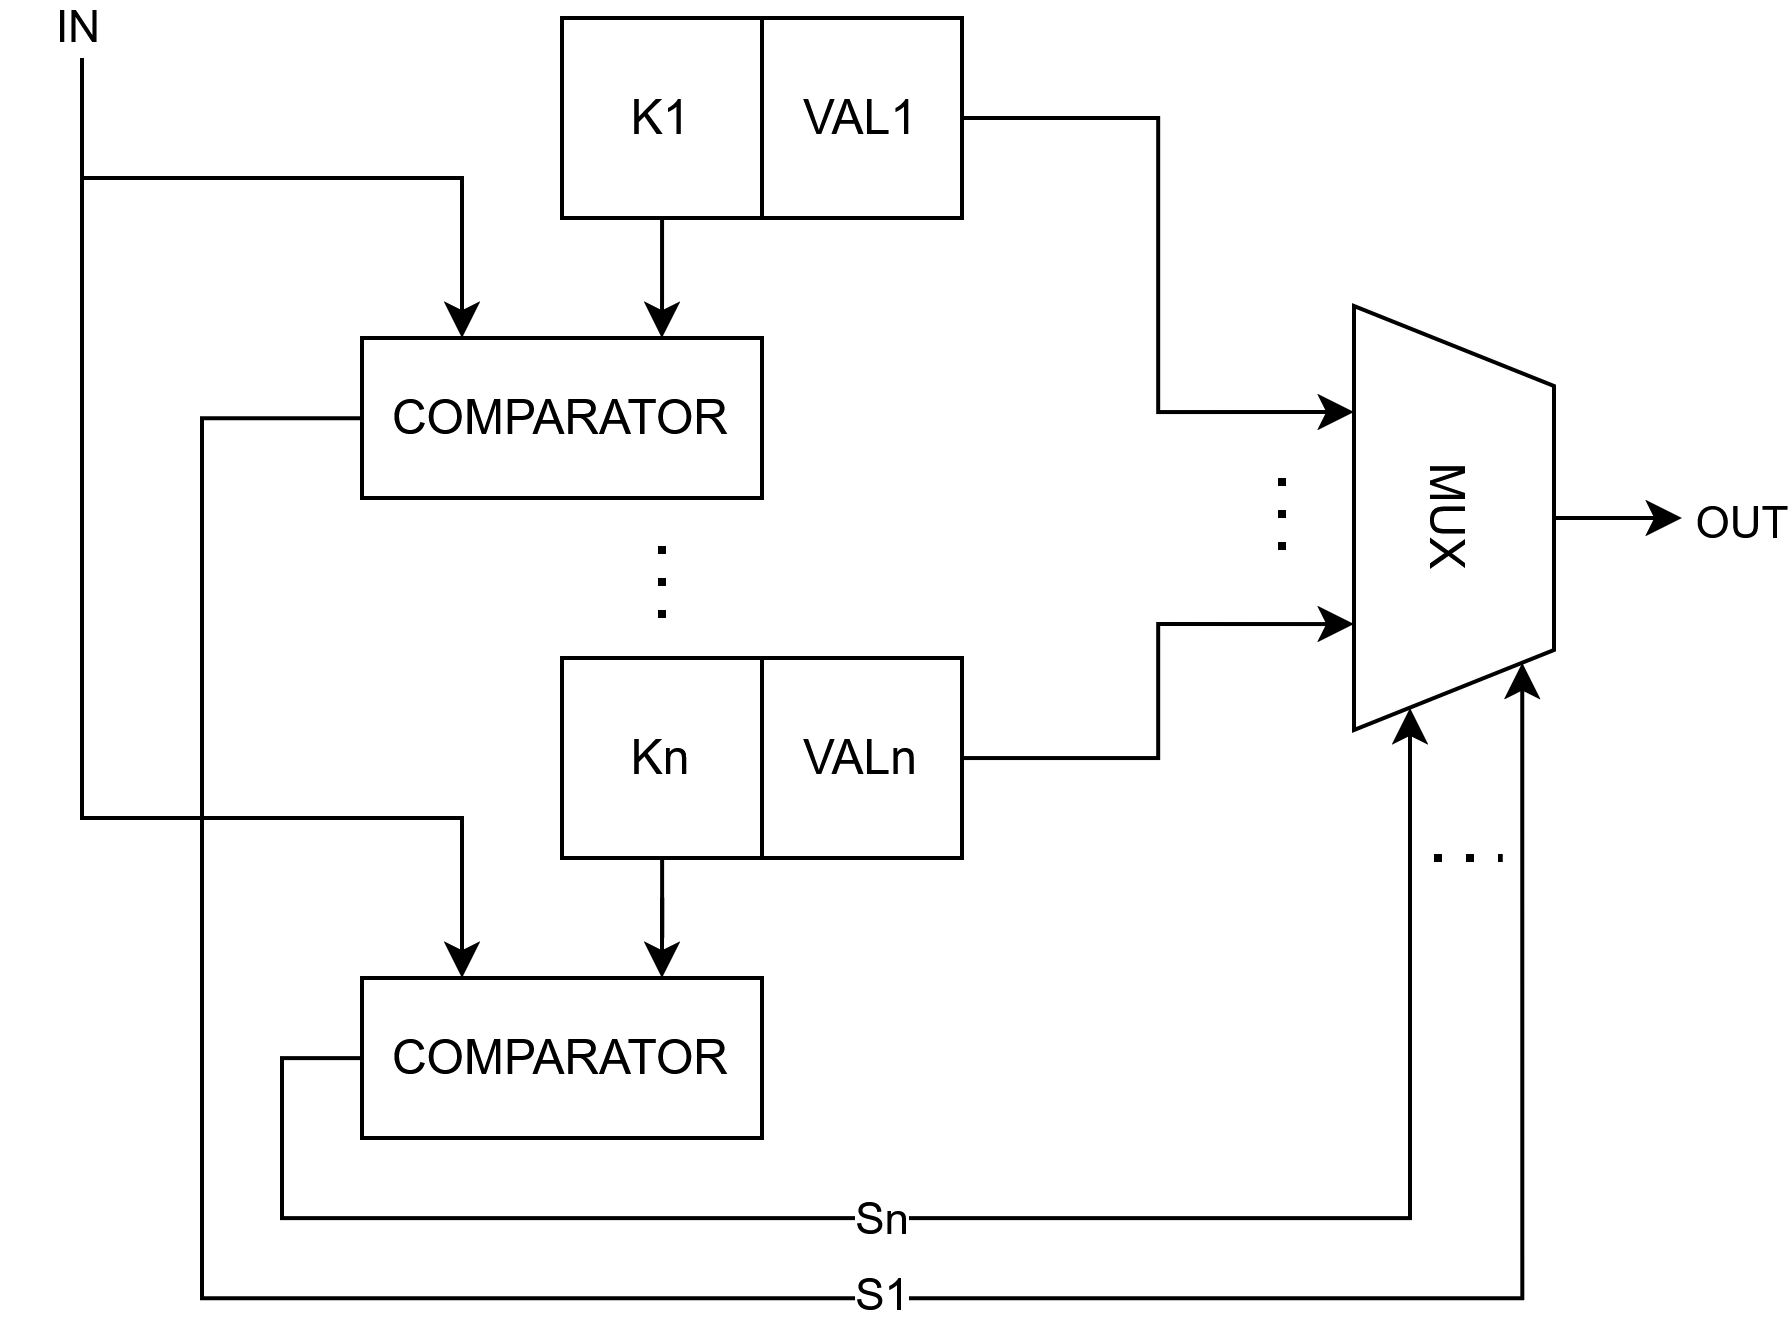
\includegraphics[width=0.5\linewidth]{img/mem_associativa.png}
    \caption{Architettura di una memoria associativa.}
    \label{fig:mem_associativa}
\end{figure}

\subsection{Gestione dei conflitti sui dati}
Se due istruzioni consecutive tentano di accedere contemporaneamente ad uno stesso registro/locazione di memoria, come già accennato in precedenza, si generano \textbf{conflitti sui dati}, classificabili in \textit{Read after Write} (R/W) e \textit{Write after Read} (W/R). Le operazioni R/R e W/W, invece, non causano problemi: la prima perché la lettura non modifica lo stato dei registri/memoria, la seconda perché conta solo la scrittura operata dalla seconda istruzione. Consideriamo un esempio di conflitto R/W.
\begin{lstlisting}
i:   R2 = R1 + R3  
i+1: R4 = R2 + R5
\end{lstlisting}
La seconda istruzione (i+1) vuole leggere R2 prima che la prima (i) abbia terminato di scriverlo. Questo genererebbe uno stallo, perché la pipeline dovrebbe aspettare. Il problema viene risolto utilizzando la tecnica dell'anticipo degli operandi, anche nota come \textbf{Operand Fowarding}: il dato appena calcolato dall’ALU (fase EX della i) viene “girato” direttamente alla EX della i+1 senza aspettare che venga scritto in R2 (fase WB). Dunque, la soluzione consiste nel creare un canale hardware che renda i risultati disponibili appena l’ALU li calcola. Notiamo come questa sia realizzabile solo se si opera su registri del processore ed ogni fase impiega un solo ciclo di clock (tipico dei processori RISC).  
\\
\\
Cerchiamo di complicare leggermente il conflitto.
\begin{lstlisting}
i:   R1 = MEMA          * carico da memoria in R1.
i+1: R2 = R1 + R3       * uso R1 subito dopo.
\end{lstlisting}
L'accesso alla memoria è molto più lento di quello ai registri, dunque, anche con la tecnica di forwarding vista in precedenza non possiamo prendere un dato dalla memoria prima che sia pronto. Se i sta ancora caricando da memoria (fase MEM), la i+1 che vuole usare il contenuto di R1 non può partire se R1 non è ancora stato aggiornato. Soprattutto se il dato non è in cache, la fase di MEM può impiegare anche decine di cicli.
\\
La linea guida generale seguita dai processori con Pipeline è che la pipe non debba mai essere interrotta: lo scopo è mantenere un flusso continuo di istruzioni attraverso le varie fasi. Utilizzare la proprietà associativa e commutativa, quando possibile, permette di modificare l'ordine delle istruzioni non bloccando la pipe. La proprietà associativa consente di associare in un solo gruppo le istruzioni indipendenti tra loro; la commutativa, invece, permette di individuare i gruppi di istruzioni invertibili, ovvero la cui inversione non causa errori di esecuzione. Tutto ciò viene implementato in hardware prima della fase di Execute (EX). Se tali proprietà non dovessero essere soddisfatte, la pipe andrebbe in stallo.
\\
\\
In tal caso, è possibile adottare un'altra tecnica nota come \textbf{Internal Fowarding}, che consiste nell'ibernare temporaneamente le istruzioni bloccate (ad esempio in attesa di dati dalla memoria), sospendendo la loro esecuzione. Nel frattempo, la pipeline può continuare con le istruzioni successive. Quando l'operazione bloccata è pronta per essere completata, viene ripresa nel corretto ordine. In questa soluzione quindi, le istruzioni vengono prelevate in sequenza ma non eseguite necessariamente in sequenza. Notiamo come questo comportamento viola il modello sequenziale di Von Neumann, in cui le istruzioni dovrebbero essere eseguite nell'ordine in cui sono scritte. Un problema importante che può emergere in questo contesto è la condivisione di registri tra istruzioni diverse. Cosa succede se più istruzioni accedono allo stesso registro? Se una lo modifica mentre un'altra lo sta ancora usando, si crea un conflitto sui dati, chiamato anche \textbf{Hazard}.  Una soluzione possibile è quella di creare più copie del registro coinvolto, in modo da tenere traccia dei diversi stati dello stesso dato nel tempo. Questo può essere implementato tramite una forma di indirizzamento indiretto: ogni registro ha uno o più puntatori che indicano sezioni di memoria dedicate a contenere le vecchie versioni del registro stesso. Per funzionare correttamente, è necessario che il numero di registri fisici (cioè le copie disponibili) sia maggiore rispetto ai registri logici visibili al programmatore, in modo da evitare conflitti durante l'esecuzione in parallelo delle istruzioni.
\begin{figure}[!h]
    \centering
    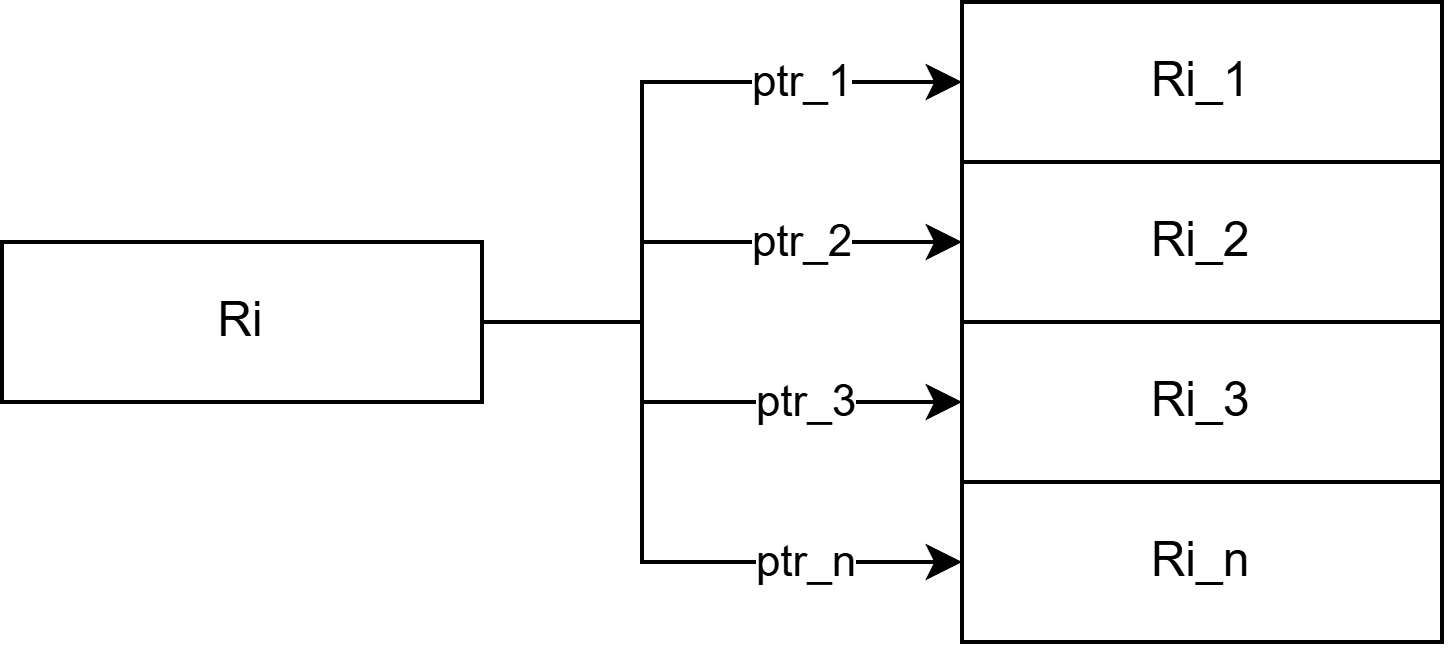
\includegraphics[width=0.4\linewidth]{img/registri_copia.png}
    \caption{Struttura dei registri copia con indirizzamento indiretto.}
    \label{fig:enter-label}
\end{figure}

\subsection{Gestione delle interruzioni}
Con l'introduzione del sistema a pipeline e del meccanismo dell'internal forwarding, che altera la sequenzialità delle istruzioni eseguite dal processore, il problema della \textbf{gestione delle interruzioni} diventa sempre più complesso. Infatti, può accadere che le istruzioni si completino in ordine diverso da quello di esecuzione. Se un'istruzione causa un'eccezione prima che le precedenti siano terminate, si parla di \textbf{interruzione non precisa}.
Per evitarlo, si mira a una \textbf{gestione precisa}, dove il sistema blocca la pipeline, completa le istruzioni precedenti e impedisce l'avvio di quelle successive, mantenendo il comportamento sequenziale previsto dal modello di Von Neumann.
\\
\\
Ricordiamo che le interruzioni sono dovute a diversi fenomeni, ma che in generale si classificano in interne ed esterne.
Le \textbf{interruzioni esterne} sono le più facili da gestire. Supponiamo di avere una pipe nella quale, in un certo momento, sono state attivate un certo numero di istruzioni. In base al modello classico di Von Neumann, occorre terminare l'operazione in corso nella pipe (e le eventuali operazioni ibernate) e salvare lo stato del processore prima di servire una interruzione. Seguendo tale modello, quindi, quando giunge un'interruzione da parte di una periferica di I/O, la ISR sarà inserita nella pipe come una qualsiasi altra istruzione. Se il sistema delle interruzioni è vettorizzato, è la stessa periferica a identificarsi mediante un numero, che il 
processore somma ad un indirizzo base, per calcolare l'indirizzo iniziale della ISR. Nel caso non vettorizzato, occorre interrogare i registri di stato di tutte le periferiche per scoprire quale ha causato l’interruzione (polling). Tale concetto si estende al caso Pipelined, salvo che le operazioni
in corso sono più di una.
\\
\\
Più critico è il caso delle \textbf{interruzioni interne}. Poiché si tratta di interruzioni che hanno effetto 
all'interno della pipe e non all'esterno, tali eventi possono dare luogo ad un comportamento del programma diverso da quello di Von Neumann. Ad esempio, potrebbe accadere che in una sequenza (i,i+1), l'istruzione i+1 generi un'eccezione prima che l'istruzione i abbia il tempo di essere eseguita. Per garantire che il 
comportamento del sistema, in queste condizioni, sia quello di Von Neumann, occorre complicare in maniera notevole l'hardware. Esempi di soluzioni che possono essere adottate sono:
\begin{itemize}
    \item \textbf{Rinuncia alle interruzioni precise}: Si accetta l'esecuzione non sequenziale, dando priorità all'interruzione che arriva per prima. Così facendo, si demanda al software la decisione sul capire se ci sono eventuali altre istruzioni in pipe che possono interrompere. È poco efficiente, ma accettabile dato che le eccezioni sono rare.
    \item \textbf{Ricostruzione delle interruzioni precise}: Le istruzioni possono essere \textit{out-of-order}, ma si impiegano due possibili approcci:
    \begin{enumerate}
        \item Nell'approccio \textit{conservativo}, ogni istruzione prosegue solo se è sicuro che non causerà eccezioni. Questo riduce il parallelismo, ma garantisce precisione.
        \item In quello \textit{ottimistico}, il processore prosegue comunque e, in caso di errore, effettua un \textbf{roll-back} (ripristino dello stato precedente). Questo richiede però di salvare lo stato del sistema.
    \end{enumerate}
\end{itemize}
Concentriamoci sulla seconda soluzione e introduciamo le due principali tecniche che permettono di implementare il roll-back.
\begin{enumerate}
    \item La tecnica del \textbf{Check Point} consiste nel salvare periodicamente lo stato del processore (sia registri che Program Counter) in una memoria dedicata. In caso di eccezione, si ripristina l’ultimo stato salvato e si riprende l'esecuzione in modo sequenziale da lì. Il problema nasce nella gestione della memoria in presenza di istruzioni che ne alterano il contenuto e che non si sarebbero dovute eseguire perché successive all'istruzione che ha generato l'eccezione.
    La principale difficoltà sta nello scegliere ogni quanto salvare i checkpoint: effettuandoli troppo spesso si rischia il sovraccarico, mentre effettuandoli troppo raramente il lavoro da fare in caso di errore aumenta.
    \item La tecnica dell'\textbf{History Buffer}, invece, utilizza un area di memoria (buffer) in cui conserva ogni istruzione eseguita insieme ai valori originali dei registri (o operandi) che modifica. Le istruzioni rimangono nel buffer finché non è certo che tutte le precedenti sono andate a buon fine (cioè non hanno generato eccezioni). Se un’eccezione si verifica, il sistema può eseguire un'operazione di UNDO per annullare gli effetti di tutte le istruzioni successive a quella che ha causato l'errore. Anche in questo caso, per garantire un’interruzione precisa, è necessario procedere in modo sequenziale durante il recupero. Il buffer utilizzato deve essere grande quanto il numero di istruzioni che possono generare contemporaneamente interruzioni. Inoltre, la gestione History Buffer non costa nulla in assenza di interruzioni, questo perché le opreazioni di memorizzazione del "vecchio stato" avvengono in parallelo alle normali operazioni del processore. Dunque, il tutto è implementato in hardware.
\end{enumerate}

In un approccio basato sul roll-back è fondamentale essere conservativi sulla scrittura in memoria, ovvero bisogna fare attenzione a non scrivere (fase WB) troppo presto. Se lo si fa e poi si scopre che un'istruzione successiva ha generato un'eccezione, la scrittura sarebbe già avvenuta e non potremmo più tornare indietro in modo pulito.

\section{Architetture Superscalari}
L'utilizzo delle pipe porta dei vantaggi non in termini di attraversamento di una istruzione, che rimane invariato, ma in termini di produttività. Per ottenere prestazioni ancora migliori, è possibile realizzare un'architettura con più pipe che eseguono diverse istruzioni in parallelo, così da aumentare la produttività del sistema. Una tale architettura viene chiamata \textbf{Superscalare}. Tuttavia, questa introduce delle problematiche che vanno necessariamente risolte, queste sono:
\begin{enumerate}
    \item Le pipe devono condividere un unico accesso in memoria comune per il prelievo delle istruzioni. In altre parole, anche in presenza di più pipe tutte devono leggere dalla stessa memoria. Questo può creare un collo di bottiglia, perché solo una pipeline alla volta può leggere da lì.
    \item Se le pipe non sono del tutto indipendenti ma condividono delle stazioni, nascono dei problemi di conflitto nell'utilizzo delle unità funzionali condivise. Se due pipeline vogliono usare la stessa unità (ad esempio, la ALU) allo stesso momento, nasce un collisione e una delle due deve aspettare. Questo riduce l'efficienza.
\end{enumerate}

\subsection{Gestione delle Collisioni}
La \textbf{gestione delle collisioni} nella architetture superscalari avviene completamente in hardware. Per comprendere al meglio come un processore con una tale architettura gestisca il problema, introduciamo un esempio. Supponiamo che la CPU sia in grado di realizzare addizione e moltiplicazione in floating point. Come possiamo immaginare, alcune delle operazioni presenti nell'addizione potrebbero essere richieste anche dalla moltiplicazione (e viceversa), mappiamo dunque all'interno di una tabella le diverse operazioni necessarie a completare le due [\ref{tab:mul} e \ref{tab:add}].

\begin{table}[!h]
\centering
\begin{tabular}{|l|c|c|c|c|c|c|c|}
\hline
         & 1 & 2 & 3 & 4 & 5 & 6 & 7 \\
\hline
Ex Add   & X &   &   &   &   &   &   \\
\hline
Mult     &   & X & X &   &   &   &   \\
\hline
Man Add  &   &   & X & X &   &   &   \\
\hline
Renorm   &   &   &   &   & X &   & X \\
\hline
Round    &   &   &   &   &   & X &   \\
\hline
Shift A  &   &   &   &   &   &   &   \\
\hline
Lead 1   &   &   &   &   &   &   &   \\
\hline
Shift B  &   &   &   &   &   &   &   \\
\hline
\end{tabular}
\caption{7 stadi richiesti dalla moltiplicazione.}
\label{tab:mul}
\end{table}

\begin{table}[!h]
\centering
\begin{tabular}{|l|c|c|c|c|c|c|c|c|c|}
\hline
         & 1 & 2 & 3 & 4 & 5 & 6 & 7 & 8 & 9 \\
\hline
Ex Add   & X &   &   &   &   &   &   &   &   \\
\hline
Mult     &   &   &   &   &   &   &   &   &   \\
\hline
Man Add  &   &   &   & X &   &   &   &   &   \\
\hline
Renorm   &   &   &   &   &   &   &   &   & X \\
\hline
Round    &   &   &   &   &   &   &   & X &   \\
\hline
Shift A  &   & X & X &   &   &   &   &   &   \\
\hline
Lead 1   &   &   &   &   & X &   &   &   &   \\
\hline
Shift B  &   &   &   &   &   & X & X &   &   \\
\hline
\end{tabular}
\caption{9 stadi richiesti dall'addizione.}
\label{tab:add}
\end{table}

L'introduzione di tali tabelle semplifica notevolmente la scrittura del \textbf{vettore delle collisioni}, ovvero un particolare vettore binario utilizzato dal compilatore per gestire il problema dei conflitti tra pipe. Poniamoci nell'ipotesi semplificativa di due sole pipe, in modo da visualizzare pù facilmente il processo. Per ricavare il vettore, è sufficiente sovrapporre le tabelle delle operazioni che vogliamo eseguire, opportunamente shiftate a seconda di quale delle due sia eseguita prima. Ad esempio, se vogliamo eseguire una moltiplicazione X e al ciclo di clock successivo un'altra moltiplicazione Y, la sovrapposizione delle tabelle fornisce il seguente risultato [\ref{tab:collision}].

\begin{table}[!h]
\centering
\begin{tabular}{|l|c|c|c|c|c|c|c|}
\hline
         & 1 & 2 & 3 & 4 & 5 & 6 & 7 \\
\hline
Ex Add   & X & Y &   &   &   &   &   \\
\hline
Mult     &   & X & XY & Y &   &   &   \\
\hline
Man Add  &   &   & X & XY & Y &   &   \\
\hline
Renorm   &   &   &   &   & X & Y & X \\
\hline
Round    &   &   &   &   &   & X & Y \\
\hline
Shift A  &   &   &   &   &   &   &   \\
\hline
Lead 1   &   &   &   &   &   &   &   \\
\hline
Shift B  &   &   &   &   &   &   &   \\
\hline
\end{tabular}
\caption{Collisioni tra due moltiplicazioni sfasate di 1 ciclo di clock.}
\label{tab:collision}
\end{table}
La tabella evidenzia come le due operazioni, eseguite secondo la tempificazione descritta, presentano delle collisioni al tempo 3 e 4 (presenza contemporanea di X e Y). Il corrispondente vettore delle collisioni sarà dunque 0011000. \MakeUppercase{è} fondamentale ribadire che il vettore si limita solamente a segnalare la presenza di una collisione (1 nella stringa), ma ciò non ha niente a che vedere con le fasi della pipeline. In altre parole, se nella stringa c'è un 1 nella terza posizione, questo NON significa che la collisione riguarda la terza fase.
\\
\\
\MakeUppercase{è} da notare come in tal caso non valga la proprietà commutativa, realizzando infatti prima una moltiplicazione e poi un'addizione non ci sarebbe alcune collisione. Nel nostro esempio ci siamo fermati a realizzare il collision vector per 1 solo caso, ovvero quello in cui una moltiplicazione segue una moltiplicazione. In generale, è necessario costruirlo per tutte le possibili combinazioni di operazioni (\textit{mul} segue \textit{add}, \textit{add} segue \textit{add}, eccetera). Se per ipotesi avessimo \(n\) istruzioni da realizzare, sarebbe necessario costruire \(2^n\) vettori, complicando notevolmente il lavoro del compilatore.
\\
\\
Ritorniamo all'esempio e cerchiamo di capire come il compilatore gestisca le collisioni per una generica sequenza di operazioni, che supponiamo essere: \textit{add, mul, mul}. \MakeUppercase{è} innanzitutto necessario costruire il vettore di collisione per le operazioni \textit{add-mul} e \textit{mul-mul}. A questo punto, bisogna inserire la seconda moltiplicazione tenendo conto sia della moltiplicazione precedente che della prima addizione. Tale condizione viene completamente gestita in hardware, secondo una struttura fatta nel seguente modo [\ref{fig:hardware-coll}].
\begin{figure}[!h]
    \centering
    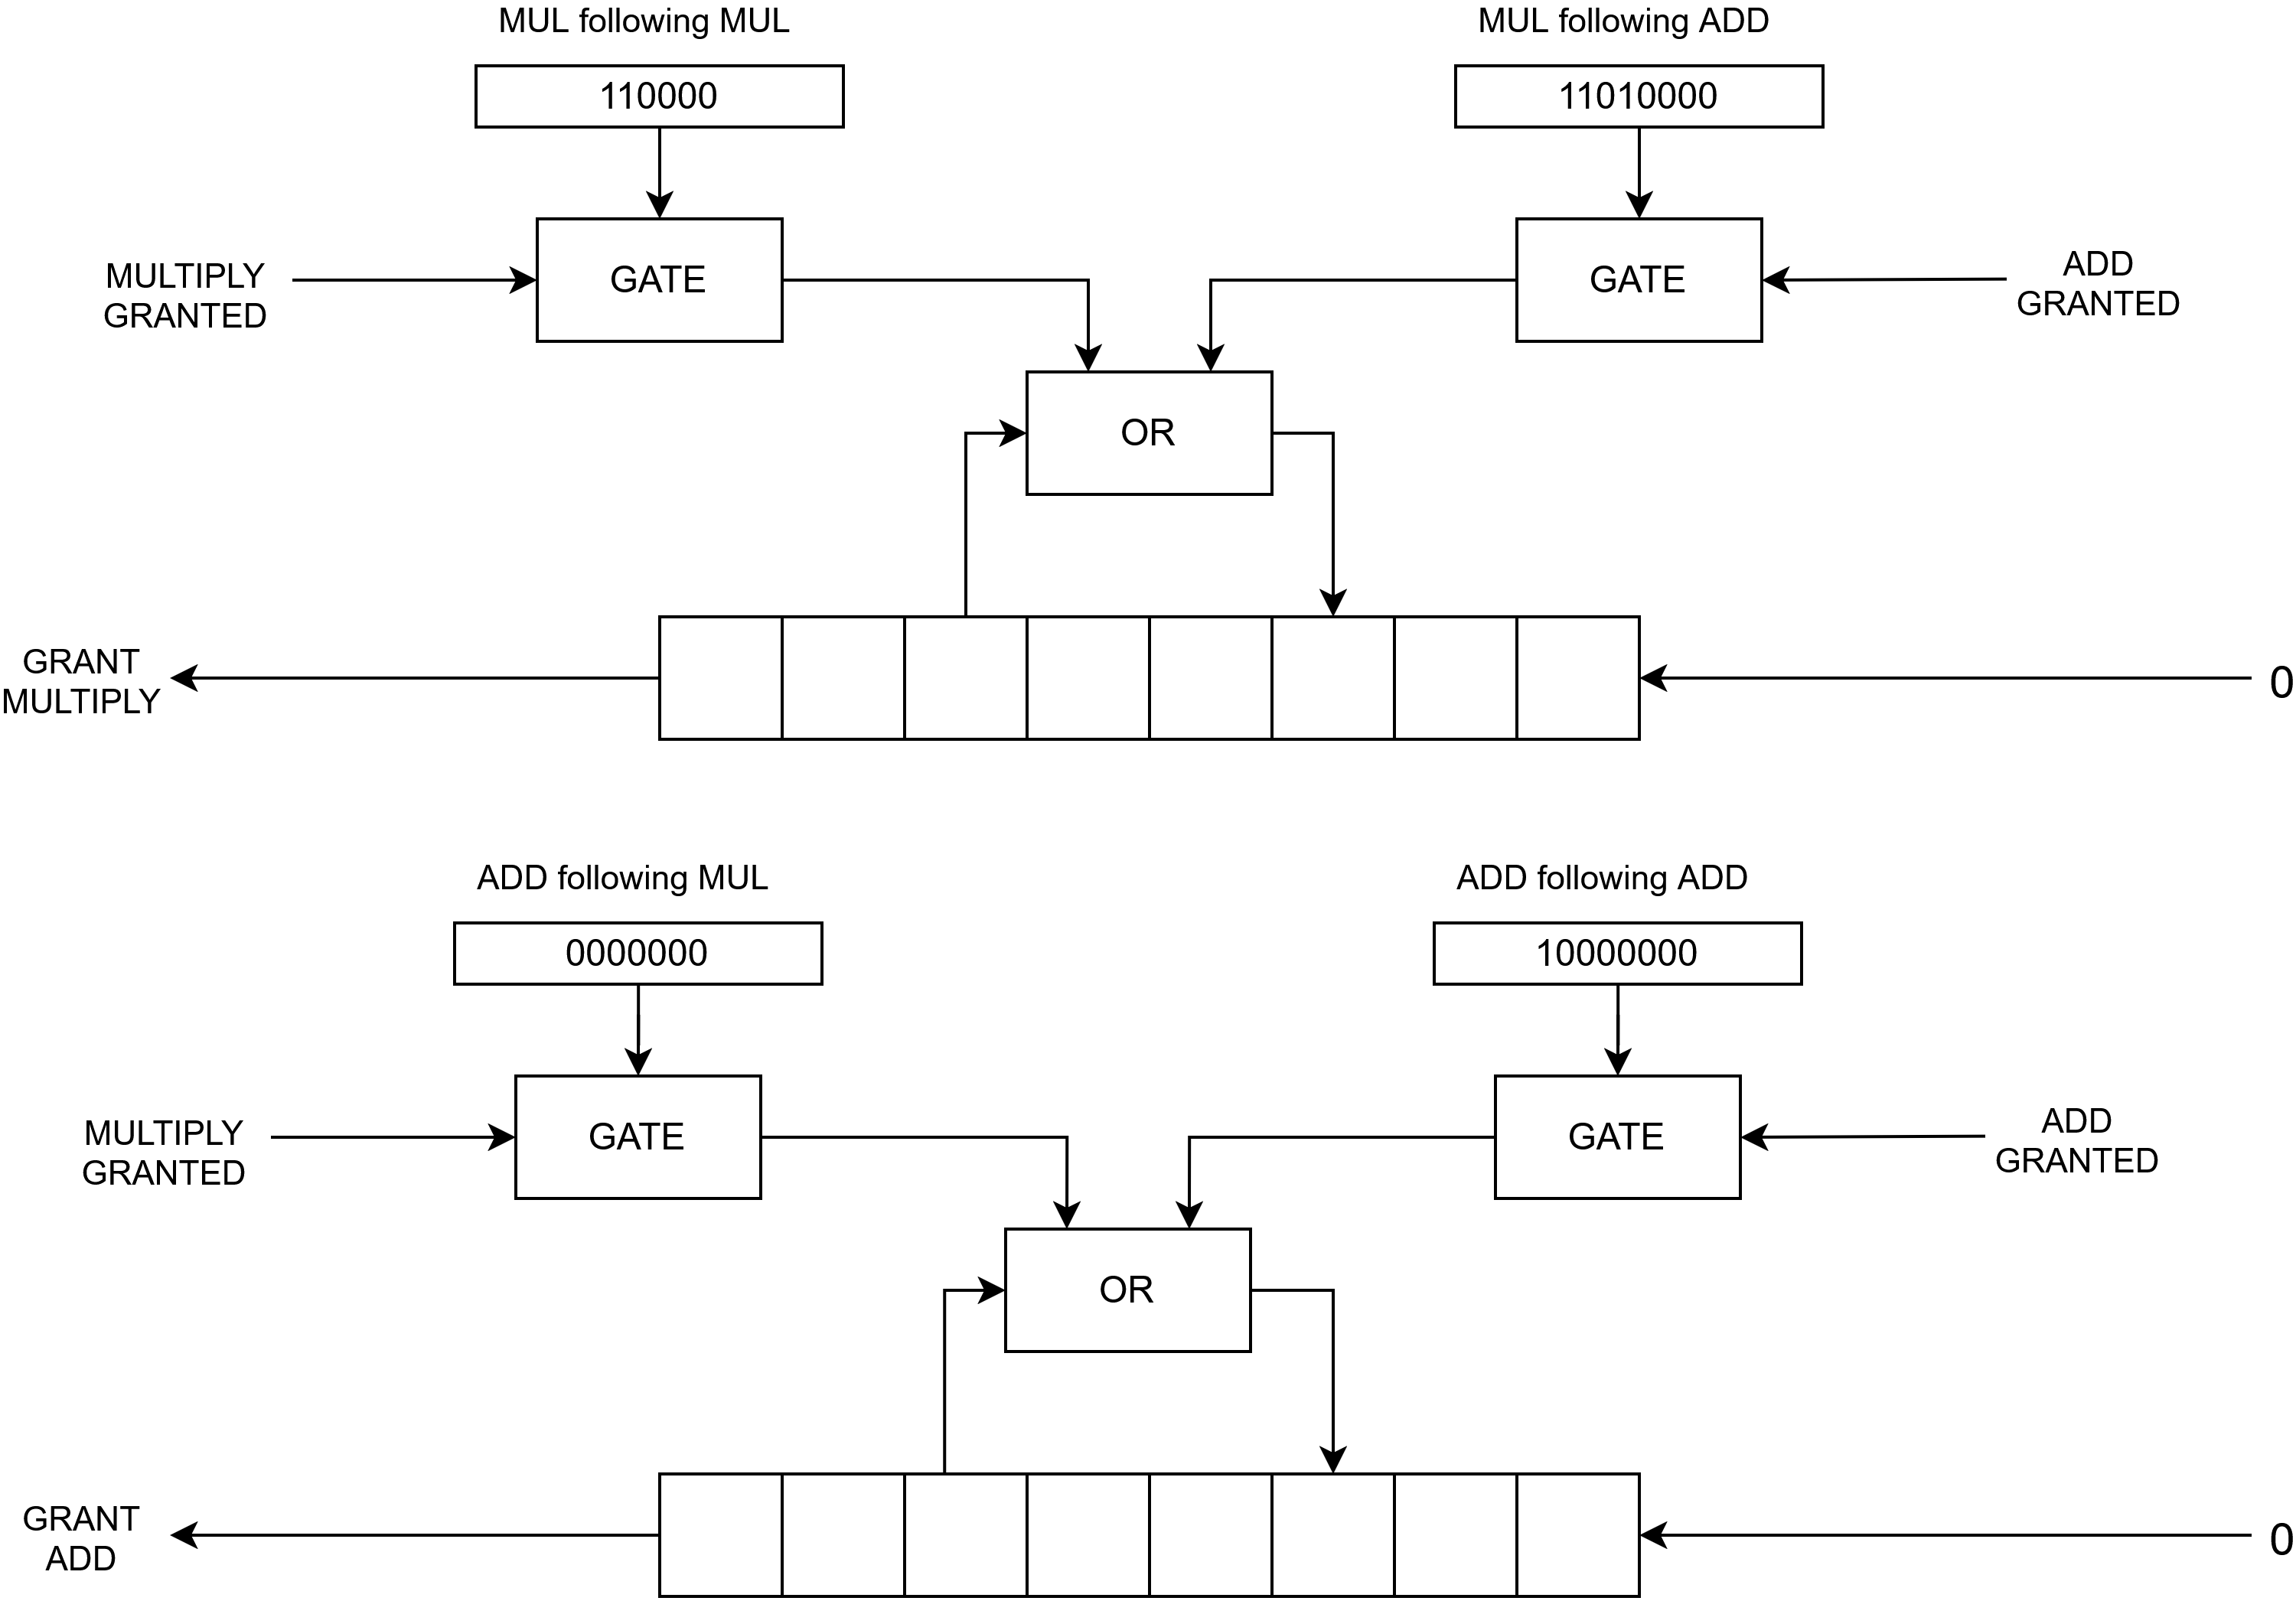
\includegraphics[width=0.7\linewidth]{img/superscalari_collisioni.png}
    \caption{Hardware per la gestione delle collisioni.}
    \label{fig:hardware-coll}
\end{figure}
In particolare, il registro a scorrimento fa proseguire la "storia" delle istruzioni, mentre la OR "unisce" la storia precedente con la nuova. Quindi, la OR garantisce che non ci sia collisione né con l'istruzione che stiamo aggiungendo, né con la storia di istruzioni precedenti. \MakeUppercase{è} fondamentale notare come la struttura sia suddivisa in due parti, quella superiore che riguarda soltanto la moltiplicazione, e quella inferiore che invece riguarda l'addizione.
\\
\\
Un tale tipo di soluzione hardware per la gestione delle collisioni è tipica dei sistemi \textbf{DSP} (Digital Signal Processor), come quelli usati per audio, video, telecomunicazioni. In particolare, il suo utilizzo permette di schedulare le istruzioni nel modo più efficiente possibile evitando stalli o rallentamenti.